\subsubsection{Schichtenmodell}

Eine der gängigsten Arten der Kommunikation findet heutzutage über das Internet statt. Dabei handelt es sich um ein weltweit verbundenes Netz von Rechnern. Zur Gewährleistung einer effizienten und geregelten Datenübertragung der heterogenen Computer im Internet wurden Regelwerke, die sogenannten Netzwerkprotokolle, benötigt. Um das Jahr 1980 wurden daraufhin von verschiedenen Computerherstellern modularisierte Protokolle entwickelt, die fortan als Standard für die digitale Übertragung innerhalb von Rechnernetzen gelten sollen. [1.0] Es musste eine Vielzahl von Aufgaben bewältigt und Anforderung bezüglich Zuverlässigkeit, Sicherheit, Effizienz etc. erfüllt werden. Die Aufgaben reichten dabei von der elektronischen Übertragung der Signale bis zur geregelten Reihenfolge der in der Kommunikation abstrakteren Aufgaben.  [1.05] Aus den zu lösenden Problemen und Anforderung kristallisierten sich sieben Schichten bzw. Ebenen heraus. Jede einzelne Schicht setzt dabei separat eine Anforderung um und kann dabei durch verschiedene Protokolle realisiert werden. In dem sich etablierten OSI-Schichtenmodell bauen die einzelnen Schichten aufeinander auf, wobei die unterste Schicht das Fundament ist. Die Open Systems Interconnection (OSI) wurde von der International Organization for Standardization (ISO), der Internationalen Organisation für Normung, als Grundlage für die Bildung von offenen Kommunikationsstandards entworfen. 
\newline

Zusätzlich zum OSI-Modell existiert das in den 1960er-Jahren entwickelte TCP/IP-Referenzmodell. Entwickler dieses Schichtmodells war das das Verteidigungsministerium der Vereinigten Staaten, auch bekannt als das Departments of Defense (DoD). Dementsprechend trägt das TCP/IP-Referenzmodell auch den Namen DoD-Schichtenmodell. [1.06]

\begin{figure}[h]
\centering
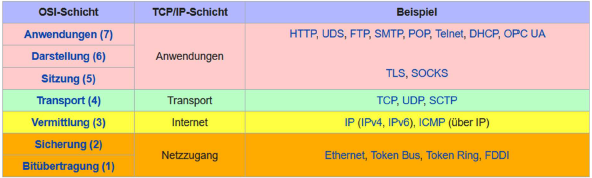
\includegraphics[width=\textwidth]{images/Netzwerkprotokolle_OSI-Schicht.PNG}
\caption{OSILAYER [1.1]}
\end{figure}

\newpage

\begin{table}[]
\begin{center}
    \begin{tabular}{| l | p{8cm} |}
    \hline
     OSI-Schicht & Aufgabe \\ 
     \hline
        
       Anwendungen & Funktionen für Anwendungen, sowie die Dateneingabe und -ausgabe. \\
    \hline    
       Darstellung & Umwandlung der systemabhängigen Daten in ein unabhängiges Format.  \\
    \hline   
       Sitzung & Steuerung der Verbindungen und des Datenaustauschs.  \\
    \hline  
        Transport & Zuordnung der Datenpakete zu einer Anwendung. \\ 
    
    \hline     
    	Vermittlung & Routing der Datenpakete zum nächsten Knoten. \\
	
    \hline       
      Sicherung & Fehlererkennungsmechanismen / Segmentierung der Pakete in Frames und Hinzufügen von Prüfsummen.  \\   
    \hline
    
    Bitübertragung & Umwandlung der Bits in ein zum Medium passendes Signal und physikalische Übertragung.\\ 
    \hline    
    \end{tabular}
\end{center}
\caption{Kurzbeschreibung der OSI-Schichten [1.2]}
\end{table}

\textbf{IP}
\newline
In der Vermittlungsschicht des OSI-Schichtenmodells findet, unabhängig des Übertragungsmediums und der genutzten Topologie, die logische Adressierung der Endgeräte statt. Das geläufigste Protokoll dafür ist das Internet Procotol (IP). Jedem am Netz verbundenen Teilnehmer wird eine IP-Adresse zugewiesen. Die bekannteste Notation ist die 32 Bit lange IPv4-Adressen und die IPv6-Adressen mit einer Größe von 128 Bit. 
\newline

\textbf{TCP/UDP}
\newline
In der Transportschicht wird eine Ende-zu-Ende-Kommunikation ermöglicht. Sie ist das Bindeglied zwischen den anwendungsorientierten und den transportorientierten Schichten. Die geläufigsten Protokolle sind das verbindungslose, unzuverlässige, aber weniger Overhead belastete User Datagram Protocol (UDP) und das verbindungsorientierte und datentransferzuverlässige Transmission Control Protocol (TCP).

\subsubsection{HTTP}
Das Hypertext Transfer Protocol, kurz HTTP, ist ein zustandloses Protokoll zur Übertragung von Daten auf der Anwendungsschicht.
\newline
\newline
\textbf{Kommunikation}
\newline
Unter einer Nachricht versteht man die HTTP die Kommunikationseinheiten zwischen dem Zentralrechner (Server) und dem, der einen Dienst vom Server abruft (Client). Man unterscheidet dabei zwischen der Anfrage (Request) vom Client an den Server und der Antwort (Response) als Reaktion vom Server zum Client. 
\newline

Eine Nachricht besteht aus dem Nachrichtenkopf (Message Header, kurz Header) und dem Nachrichtenrumpf (Message Body, kurz Body). Der Header enthält generelle Informationen über die Nachricht wie zum Beispiel den Methodentyp, das Datenformat, den genutzten Kompressionsalgorithmus, die Länge der Nachricht oder die verwendete Kodierung im Body. 
\newline

Die erste Zeile des Nachrichtenkops ist dreiteilig und besteht bei der Anfrage aus dem Namen der Anfragemethode, dem Pfad zur angeforderten Ressource (Uniform Resource Locator, kurz URL) und der verwendet HTTP-Version. Die Anfangszeile einer HTTP-Antwort dagegen besteht zunächst aus der verwendeten HTTP-Version, gefolgt von dem zweiteiligem Status-Code. Anschließend folgt eine Reihe von Headerzeilen, wobei jede Zeile aus einem Schlüsselwort/Wert-Paar besteht und die für die Datenübertragung wichtigen Informationen übergibt. Der Nachrichtenrumpf, der mit den Nachrichtenkopf über einen Zeilenumbruch syntaktisch voneinander getrennt wird, enthält schließlich die Nutzdaten. TODO BILD
\newline

\begin{figure}[h]
\centering
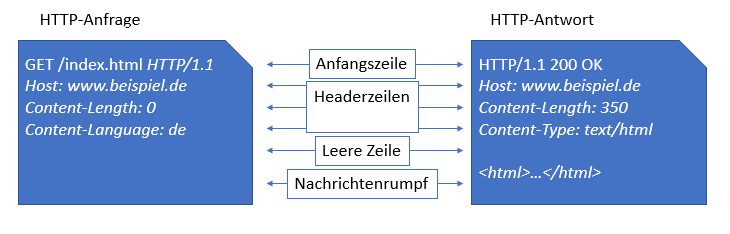
\includegraphics[width=\textwidth]{images/netzwerkprotokolle_http.PNG}
\caption{HTTP-Nachrichtenaufbau}
\end{figure}

\textbf{Methoden}
\newline
HTTP bietet fest definierte Standard-Methoden für Anfragen, die für verschiedene Aufgaben gedacht sind. Im Folgenden werden die wichtigsten Methoden beschrieben:
\newline

\begin{enumerate}
		\item \textit{GET} ist die gebräuchlichste Methode. Sie fordert vom Server eine Ressource, die bei Erfolg in der Antwort im Body zurückgegeben wird. 
		
		\item \textit{POST} ist für die Änderung oder Erzeugung einer Ressource vorgesehen. Dafür werden bei der Anfrage zusätzlich Daten im Body der Nachricht übertragen.
		
		\item \textit{PUT} dient dazu, eine Ressource zu verändern, oder bei Nichtexistenz zu erstellen.
	
		\item \textit{PATCH} ändert eine bestehende Ressource ohne diese wie bei PUT vollständig zu ersetzen. 
		
		\item \textit{DELETE} löscht die angegebene Ressource auf dem Server.
		
		\item \textit{OPTIONS} liefert eine Liste von Methoden und Merkmale, die vom Server unterstützt werden.
		
\end{enumerate}

\textbf{Statuscodes}
\newline
HTTP-Antworten senden in der Anfangszeile ihrer Nachricht Statuscodes. Die Angabe ist zweiteilig und besteht aus einer standardisierten Statuskennzahl sowie einer kurzen textuellen Beschreibung, die zusammen Auskunft über den Bearbeitungszustand der zugehörigen Anfrage geben.\newline

\begin{figure}[h]
\centering
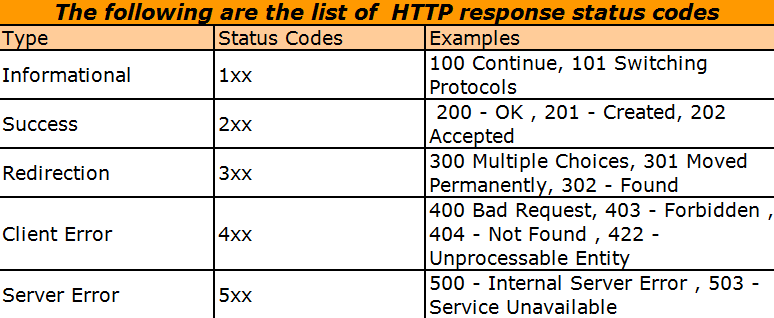
\includegraphics[width=\textwidth]{images/netzwerkprotokolle_Httpstatuscodes.png}
\caption{HTTP-Statuscodes}
\end{figure}

\newpage
\subsubsection{HTTPS}
Lorem ipsum dolor sit amet, consetetur sadipscing elitr, sed diam nonumy eirmod tempor invidunt ut labore et dolore magna aliquyam erat, sed diam voluptua. At vero eos et accusam et justo duo dolores et ea rebum. Stet clita kasd gubergren, no sea takimata sanctus est Lorem ipsum dolor sit amet. Lorem ipsum dolor sit amet, consetetur sadipscing elitr, sed diam nonumy eirmod tempor invidunt ut labore et dolore magna aliquyam erat, sed diam voluptua. At vero eos et accusam et justo duo dolores et ea rebum. Stet clita kasd gubergren, no sea takimata sanctus est Lorem ipsum dolor sit amet.